\documentclass{article}
\usepackage{tikz}
\usetikzlibrary{arrows.meta, calc}

% Define some styles for consistency
\tikzset{
    >=Stealth, % Arrowhead style
    line width=1pt, % Line thickness
    blue line/.style={blue!70!black, line width=1.2pt}, % Blue lines for emphasis
    black line/.style={black, line width=1pt}, % Black lines for standard strokes
    arrow label/.style={font=\footnotesize, above=3pt, sloped}, % Style for arrow labels
}

\begin{document}

\begin{figure}[ht]
    \centering
    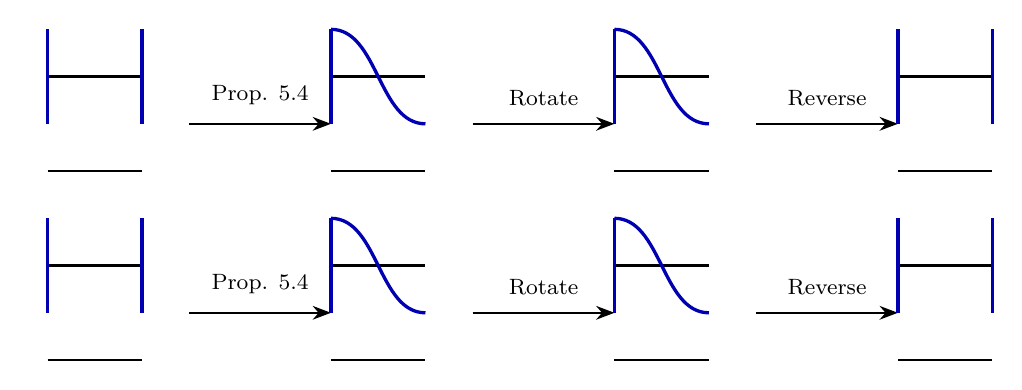
\begin{tikzpicture}[scale=1.2]

    % First row
    \begin{scope}[local bounding box=row1]
        % First diagram
        \draw[black line] (-1.5,0) -- (-0.5,0);
        \draw[black line] (-1.5,-1) -- (-0.5,-1);
        \draw[black line] (-1.5,-0.5) -- (-1.5,-0.5) node[left] {$ $};
        \draw[blue line] (-1.5,-0.5) -- (-1.5,0.5);
        \draw[blue line] (-0.5,-0.5) -- (-0.5,0.5);

        % Arrows and labels
        \draw[->, thick] (0, -0.5) -- node[arrow label] {Prop. 5.4} (1.5, -0.5);

        % Second diagram
        \begin{scope}[shift={(3,0)}]
            \draw[black line] (-1.5,0) -- (-0.5,0);
            \draw[black line] (-1.5,-1) -- (-0.5,-1);
            \draw[black line] (-1.5,-0.5) -- (-1.5,-0.5) node[left] {$ $};
            \draw[blue line] (-1.5,-0.5) -- (-1.5,0.5);
            \draw[blue line] (-0.5,-0.5) .. controls +(-0.5,0) and +(0.5,0) .. (-1.5,0.5);

            % Arrows and labels
            \draw[->, thick] (0, -0.5) -- node[arrow label] {Rotate} (1.5, -0.5);
        \end{scope}

        % Third diagram
        \begin{scope}[shift={(6,0)}]
            \draw[black line] (-1.5,0) -- (-0.5,0);
            \draw[black line] (-1.5,-1) -- (-0.5,-1);
            \draw[black line] (-1.5,-0.5) -- (-1.5,-0.5) node[left] {$ $};
            \draw[blue line] (-1.5,-0.5) -- (-1.5,0.5);
            \draw[blue line] (-1.5,0.5) .. controls +(0.5,0) and +(-0.5,0) .. (-0.5,-0.5);

            % Arrows and labels
            \draw[->, thick] (0, -0.5) -- node[arrow label] {Reverse} (1.5, -0.5);
        \end{scope}

        % Fourth diagram
        \begin{scope}[shift={(9,0)}]
            \draw[black line] (-1.5,0) -- (-0.5,0);
            \draw[black line] (-1.5,-1) -- (-0.5,-1);
            \draw[black line] (-1.5,-0.5) -- (-1.5,-0.5) node[left] {$ $};
            \draw[blue line] (-1.5,-0.5) -- (-1.5,0.5);
            \draw[blue line] (-0.5,0.5) -- (-0.5,-0.5);
        \end{scope}
    \end{scope}

    % Second row
    \begin{scope}[yshift=-2cm]
        \begin{scope}[local bounding box=row2]
            % First diagram
            \draw[black line] (-1.5,0) -- (-0.5,0);
            \draw[black line] (-1.5,-1) -- (-0.5,-1);
            \draw[black line] (-1.5,-0.5) -- (-1.5,-0.5) node[left] {$ $};
            \draw[blue line] (-1.5,-0.5) -- (-1.5,0.5);
            \draw[blue line] (-0.5,-0.5) -- (-0.5,0.5);

            % Arrows and labels
            \draw[->, thick] (0, -0.5) -- node[arrow label] {Prop. 5.4} (1.5, -0.5);

            % Second diagram
            \begin{scope}[shift={(3,0)}]
                \draw[black line] (-1.5,0) -- (-0.5,0);
                \draw[black line] (-1.5,-1) -- (-0.5,-1);
                \draw[black line] (-1.5,-0.5) -- (-1.5,-0.5) node[left] {$ $};
                \draw[blue line] (-1.5,-0.5) -- (-1.5,0.5);
                \draw[blue line] (-0.5,-0.5) .. controls +(-0.5,0) and +(0.5,0) .. (-1.5,0.5);

                % Arrows and labels
                \draw[->, thick] (0, -0.5) -- node[arrow label] {Rotate} (1.5, -0.5);
            \end{scope}

            % Third diagram
            \begin{scope}[shift={(6,0)}]
                \draw[black line] (-1.5,0) -- (-0.5,0);
                \draw[black line] (-1.5,-1) -- (-0.5,-1);
                \draw[black line] (-1.5,-0.5) -- (-1.5,-0.5) node[left] {$ $};
                \draw[blue line] (-1.5,-0.5) -- (-1.5,0.5);
                \draw[blue line] (-1.5,0.5) .. controls +(0.5,0) and +(-0.5,0) .. (-0.5,-0.5);

                % Arrows and labels
                \draw[->, thick] (0, -0.5) -- node[arrow label] {Reverse} (1.5, -0.5);
            \end{scope}

            % Fourth diagram
            \begin{scope}[shift={(9,0)}]
                \draw[black line] (-1.5,0) -- (-0.5,0);
                \draw[black line] (-1.5,-1) -- (-0.5,-1);
                \draw[black line] (-1.5,-0.5) -- (-1.5,-0.5) node[left] {$ $};
                \draw[blue line] (-1.5,-0.5) -- (-1.5,0.5);
                \draw[blue line] (-0.5,0.5) -- (-0.5,-0.5);
            \end{scope}
        \end{scope}
    \end{scope}

    \end{tikzpicture}
    \caption{The saddle moves of Proposition \ref{prop:newii} are consistent under mirror image, as explained in the proof of Proposition \ref{prop:newimirror}.}
\end{figure}

\end{document}